\section{示例：建立低維模型}\label{sec:nanostructure-examples}
\index{Namidai@奈米帶}\index{Namiguan@奈米管}\index{Namixian@奈米線}

把片層裁成帶，或沿一個方向捲成管，會改變結構的邊界和週期。奈米帶在寬度方向出現邊緣，只沿長度方向重複；奈米管沿軸向重複，另外兩個方向留出真空。由塊體擷取的奈米線也只有一個週期方向；有限團簇則在三個方向都不重複。

本節先用一份小的石墨烯原胞建立24位點奈米帶和32位點奈米管，再從面心立方銅建立奈米線、有限團簇和球形空洞。每個結果都配有原生JSON與CIF檔案，可一邊構建，一邊與隨書結果比較。

\subsection{準備六十度石墨烯原胞}

隨書\file{nano-graphene-60.json}含兩個C位點，面內兩個晶格向量長度均為 $2.46\,\text{\AA}$，夾角 $60^\circ$，法向盒高 $15\,\text{\AA}$；兩個面內方向週期，法向非週期。它與前面的\file{graphene-layer.json}表示同一張石墨烯，區別是晶格基底的選取。

若從前面的 $120^\circ$ 原胞出發，可保留 $\mathbf a$，將第二個向量換成 $\mathbf a+\mathbf b$。新向量仍長 $2.46\,\text{\AA}$，但與 $\mathbf a$ 的夾角成為 $60^\circ$。這次整數換基的行列式為1，因此不會擴大模型，仍有兩個獨立位點。本節的帶和管均使用這份 $60^\circ$ 輸入。

\begin{steps}
  \item 將\file{nano-graphene-60.json}匯入專案，命名為\file{nano-graphene}，開啟三維文件，檢查兩個獨立位點、等長的面內晶格和 $60^\circ$ 夾角。
  \item 如希望自己換基，另行匯入原始\file{graphene-layer.json}並啟用。在\ui{晶體建模}\,$\rightarrow$\,\ui{超胞與晶格}中開啟\ui{構建超胞}。
  \item 在\ui{超胞倍率或變換矩陣}文字框中輸入\literalinput{1 0 0; 1 1 0; 0 0 1}。這是三行整數矩陣，分號用於分行；與編輯晶格視窗的逐格表格不同。
  \item 預覽後核對位點數仍為2，晶胞體積保持不變，面內夾角變為 $60^\circ$。應用後另存為能說明基底的名稱，不覆蓋原來的 $120^\circ$ 單層。
  \item 為奈米帶與奈米管分別保留一份輸入。每次構建都從單層開始，不能在已經裁成帶的結果上繼續執行卷管而當作同一個例子。
\end{steps}

兩種基底的晶胞邊框看起來不同，但原材料的週期幾何相同。使用本節命令時，先核對輸入檔案與基底，再比較位點數和尺寸；只抄寫寬度或手性指數，不足以確定同一個構建過程。

\subsection{裁出一條扶手椅邊石墨烯奈米帶}

奈米帶的寬度和軸向長度按重複單元數填寫；真空以\AA 為單位。\ui{armchair}與\ui{zigzag}描述兩種不同的邊緣排列，不是兩個相機方向。這裡選擇扶手椅邊，先檢查邊緣上的碳原子怎樣成對排列，再看沿帶長方向的週期連線。

\begin{table}[htbp]
\centering\small
\caption{24位點扶手椅邊奈米帶的引數。}
\begin{tabularx}{\linewidth}{lX}
\toprule
欄位 & 本例輸入\\
\midrule
寬度方向重複單元數 & 3，無量綱整數。\\
軸向重複單元數 & 2，無量綱整數。\\
邊緣型別 & 選擇\ui{armchair}。\\
真空層厚度（Å） & 5；本工具在兩個非週期方向的兩側分別留出該空白。\\
最大原子數 & 500；是構建規模上限，不是要求最終有500個位點。\\
\bottomrule
\end{tabularx}
\end{table}

\begin{steps}
  \item 啟用準備好的\file{nano-graphene}單層。從\ui{晶體建模}的\ui{奈米結構}選單開啟\ui{擷取奈米帶}。
  \item 按表填寫引數。寬度3不是 $3\,\text{\AA}$；軸向2也不是 $2\,\text{\AA}$。
  \item 單擊\ui{預覽}，顯示晶胞邊框。沿片層法向檢視兩條邊，轉到側面確認模型仍是一張平帶。
  \item 檢查獨立位點數為24，所有原子均為C。沿週期方向檢視接續，不能把靠近晶胞兩端的同一週期網路看成兩段斷開的分子。
  \item 應用後命名為\file{graphene-armchair-w3-l2}，儲存專案，並與隨書同名JSON比較。原單層仍需單獨保留。
\end{steps}

本例輸出在全域性 $y$ 方向週期，原生週期標記為\literalinput{false true false}。三個胞長約為 $16.15$、$8.521690$、$10.00\,\text{\AA}$。其中沿帶長的週期為 $8.521690\,\text{\AA}$；原子在寬度方向的實際跨度為 $6.15\,\text{\AA}$，再加兩側各 $5\,\text{\AA}$ 空白，得到 $16.15\,\text{\AA}$ 的盒寬。平片本身沒有法向厚度，所以該方向的盒長為 $10\,\text{\AA}$。

未鈍化的24個C原子中，以 $1.65\,\text{\AA}$ 為近鄰檢查界限，有16個原子連線三個近鄰，8個邊緣原子連線兩個近鄰；最短週期原子間距約為 $1.420282\,\text{\AA}$。這個界限用於核對這組碳模型，並不是所有元素的通用成鍵距離。若要研究氫鈍化邊緣，應另存未鈍化模型，再按目標邊緣配位新增氫並檢查組成。

\subsection{把石墨烯捲成一根小奈米管}

捲曲前先確定平面中哪一條向量將成為管的圓周。幫助資訊中的幾何關係為
\begin{equation}
  \mathbf C_h=n\mathbf a_1+m\mathbf a_2,
  \qquad R=\frac{\|\mathbf C_h\|}{2\pi}.
  \label{eq:nanotube-circumference-radius}
\end{equation}
$\mathbf a_1,\mathbf a_2$是輸入片層的面內晶格向量，單位為\AA；$n,m$是無量綱手性指數，$\mathbf C_h$是手性向量，$R$為初始管半徑。圓周長度取兩個基矢線性組合的模。等長、夾角$60^\circ$的面內基矢給出$\|\mathbf C_h\|=a\sqrt{n^2+nm+m^2}$；換用其他基底時，應回到式\eqref{eq:nanotube-circumference-radius}計算。本節沿用已整理好的$60^\circ$輸入；不同基底中的同一組$(n,m)$不應直接視為同一捲曲方向。

\begin{figure}[htbp]
\centering
\begin{tikzpicture}[x=1mm,y=1mm,font=\sffamily\small,>=stealth]
  \node[text=brand] at (26,54) {平面中的卷曲方向};
  \foreach \j in {0,1,2,3} {
    \draw[teal!55] ({6+4*\j},{10+7*\j}) -- ({38+4*\j},{10+7*\j});
    \foreach \i in {0,1,2,3,4} {
      \fill[brand] ({6+8*\i+4*\j},{10+7*\j}) circle (.8);
    }
  }
  \foreach \i in {0,1,2,3,4}
    \draw[teal!55] ({6+8*\i},10) -- ({18+8*\i},31);
  \draw[->,brand,line width=.9pt] (6,10) -- (38,10)
    node[midway,below=3pt] {$\mathbf C_h=4\mathbf a_1$};
  \draw[->,muted] (6,10) -- (14,10) node[above] {$\mathbf a_1$};
  \draw[->,muted] (6,10) -- (10,17) node[left] {$\mathbf a_2$};
  \draw[->,teal,line width=.8pt] (57,24) -- (69,24);
  \node[text=muted,font=\sffamily\footnotesize] at (63,32) {卷合};
  \node[text=brand] at (95,54) {圆周长度不变};
  \fill[paleblue] (81,10) rectangle (109,39);
  \draw[brand,line width=.8pt] (81,10) -- (81,39);
  \draw[brand,line width=.8pt] (109,10) -- (109,39);
  \draw[brand,fill=paleblue,line width=.8pt] (95,39) ellipse (14 and 5);
  \draw[brand,line width=.8pt] (81,10) arc[start angle=180,end angle=360,x radius=14mm,y radius=5mm];
  \draw[brand,densely dashed] (109,10) arc[start angle=0,end angle=180,x radius=14mm,y radius=5mm];
  \draw[->,muted] (95,39) -- (109,39) node[midway,above] {$R$};
  \draw[->,teal] (115,10) -- (115,43) node[above] {管轴};
  \node[align=center,font=\sffamily\footnotesize] at (95,-1) {$\|\mathbf C_h\|=2\pi R$};
\end{tikzpicture}
\caption{手性矢量与管半径的关系（示意）。左图的点表示晶格平移点，以$(4,0)$标出卷成一周的平面方向；右图表示卷曲后圆周与半径的几何关系。}
\label{fig:nanotube-chiral-geometry}
\end{figure}


手性指數 $(n,m)$ 指定捲成圓周的晶格方向，軸向重複數決定沿管軸保留多少個平移週期。本例使用 $(4,0)$，管半徑較小，便於觀察捲曲、接縫與週期。穩定半徑需在幾何弛豫後確定。

\begin{steps}
  \item 回到原始\file{nano-graphene-60.json}，另開一份單層文件並啟用。不要使用剛生成的奈米帶。
  \item 在\ui{奈米結構}選單選擇\ui{生成奈米管}。在\ui{手性指數（n m）}的兩個數值框中分別填4與0。
  \item \ui{軸向重複單元數}設為2，\ui{真空層厚度（Å）}設為6，\ui{最大原子數}設為500。
  \item 預覽後沿管軸觀察環形截面，再從側面檢查管身。轉動相機檢視卷合位置，並核對軸向兩端能按週期相接。
  \item 檢查模型共有32個C位點。應用後儲存為\file{graphene-tube-4-0-l2}，保留單層輸入和奈米管結果。
\end{steps}

本例沿全域性 $z$ 方向週期，週期標記為\literalinput{false false true}。由捲曲圓周得到的半徑為
\[
 R=\frac{4\times2.46}{2\pi}\,\text{\AA}\approx1.566085\,\text{\AA}.
\]
兩個橫向胞長均約為 $15.132169\,\text{\AA}$，等於管直徑加兩側各 $6\,\text{\AA}$ 真空；軸向胞長約為 $8.521690\,\text{\AA}$。本工具的橫向真空與扭轉雙層視窗中的\ui{總真空層厚度}含義不同，比較盒長時應按各命令的定義計算。

對儲存座標作週期近鄰檢查，32個位點均有三個距離小於 $1.65\,\text{\AA}$ 的近鄰，最短間距約為 $1.393202\,\text{\AA}$。平片捲成很小的圓周後，兩點之間的直線距離會與平面上的距離不同。因此，不必要求卷管後的全部C--C直線距離仍恰好等於平片的 $1.420282\,\text{\AA}$；應同時檢查半徑、接縫、近鄰與週期，後續幾何弛豫另行進行。

\subsection{從管口與側面閱讀奈米管}

已構建的奈米管也可以直接從隨書\file{graphene-tube-4-0-l2.json}匯入。這樣可以先熟悉觀察方法，再回到引數視窗比較不同的手性指數。初次取景保持\ui{Input cell}與\ui{1 × 1 × 1}，使畫面對應儲存的一個模型週期。

\begin{steps}
  \item 在\ui{主頁 → 結構 → 從檔案匯入結構}中選擇該JSON；線上版先上傳，再從雲檔案匯入。開啟結構文件，確認元素為C，模型摘要為32個位點。
  \item 在檢視工具欄單擊\ui{c}，其提示為\ui{View along c axis}。本例管軸與$c$平行，因此現在從管口看向管內；觀察碳原子圍成的環和中央空心區域。
  \item 單擊\ui{a}或\ui{b}轉到側面。保持相同縮放，檢查管身沿軸向延伸，六元環在曲面上的排列仍可辨認。若球體遮住連線，在\ui{Viewer settings → Style}中適度減小\ui{Atom scale}，再檢視區域性。
  \item 在\ui{Visibility}中顯示\ui{Unit cell}，把細長的管身與橫向真空盒比較。需要看清單個週期的原子時，可先隱藏\ui{Boundary image atoms}；檢查兩端接續時再顯示邊界映像。
  \item 在\ui{Scientific scene → Repeat cell}中只把\ui{c}設為2，觀察軸向兩段怎樣接上。看完使用\ui{Reset to 1 × 1 × 1}恢復，最後單擊\ui{Reset camera}重新取全景。
  \item 分別匯出管口和側面圖片，記錄兩圖來自同一32位點結構，並註明$(4,0)$、軸向兩個重複單元及原始JSON檔名。
\end{steps}

沿管軸看見“孔”，說明當前座標圍成了管形；側面和重複顯示則幫助確認它沿軸向週期延伸。顯示重複沒有把輸入改成更大的計算超胞。邊界附近增加的球體也屬於場景映像，模型獨立位點數仍應按原始結構讀取。以這兩種取向共同說明形態，比只留一張斜檢視更容易辨認管徑、管長與週期。

\begin{figure}[!htb]
\centering
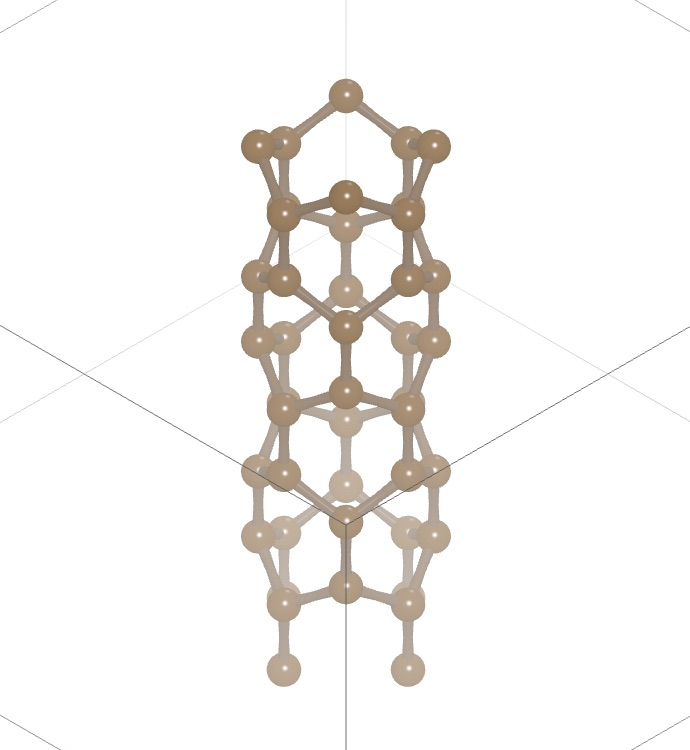
\includegraphics[width=.47\linewidth]{publication-assets/revision-nanotube-perspective.png}\hfill
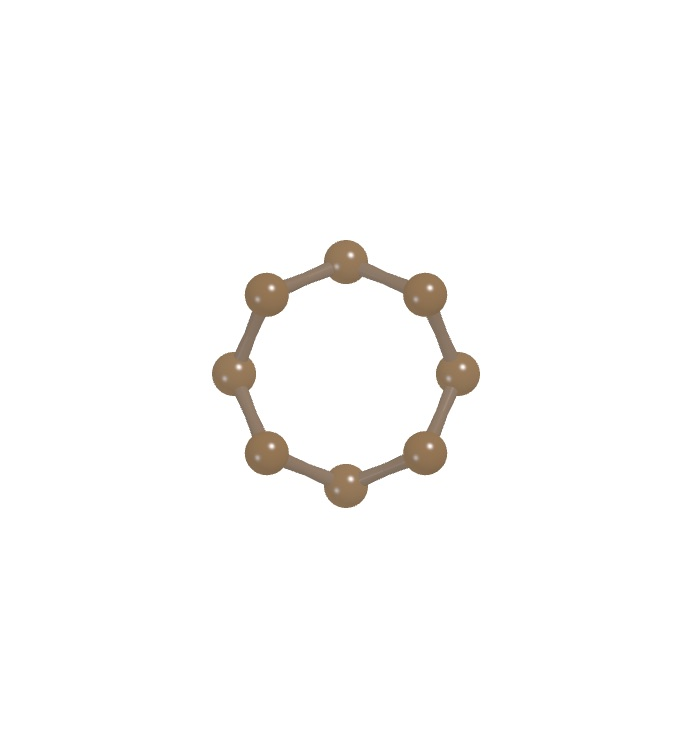
\includegraphics[width=.47\linewidth]{publication-assets/revision-nanotube-axis-c.png}
\caption{同一32位點碳奈米管的三維檢視。左：從側面檢查曲面的碳網路和軸向連線；右：沿管口方向觀察中央空心區域。顯示中包含週期邊界映像，獨立位點數保持32。}
\label{fig:nanotube-live}
\end{figure}

\FloatBarrier
\subsection{從銅晶體擷取奈米線}

銅例子使用隨書\file{nano-Cu-fcc-input.json}，與\file{Cu-fcc.cif}來自相同的四位點面心立方晶胞，晶格常數為 $3.61\,\text{\AA}$。奈米線保留一個晶格方向的平移週期，橫截面則按給定半徑擷取。擷取球或圓柱時，原子不是連續分佈的介質；實際最外原子的跨度不一定等於兩倍輸入半徑。

週期方向指數$[u\,v\,w]$透過實空間晶格給出線軸方向：
\begin{equation}
  \mathbf t=u\mathbf a+v\mathbf b+w\mathbf c.
  \label{eq:nanowire-lattice-direction}
\end{equation}
$u,v,w$為無量綱整數，$\mathbf t$與晶格向量使用相同的長度單位。構建時取與$\mathbf t$平行的軸，再以給定半徑保留橫截面內的原子；軸向週期長度以輸出晶胞為準。

\begin{table}[htbp]
\centering
\caption{晶格方向指標與晶面指標的區別。}
\begin{tabularx}{\linewidth}{lX}
\toprule
輸入 & 對應的幾何關係與用途\\
\midrule
$[u\,v\,w]$方向 & 由實空間的$\mathbf a,\mathbf b,\mathbf c$組合得到，用於奈米線軸向等方向選擇。\\
$(hkl)$晶面 & 由倒格矢組合得到法向，見式\eqref{eq:surface-miller-normal}，用於表面切割。\\
\bottomrule
\end{tabularx}
\end{table}

在立方晶胞中，同一組三個整數給出的方向與同指數晶面的法向平行；在一般斜晶胞中並非如此。填寫前先看視窗要求的是方向還是晶面，再從軸向和側向檢查預覽。

\begin{steps}
  \item 匯入銅輸入並啟用，在\ui{奈米結構}中開啟\ui{擷取奈米線}。
  \item 在\ui{週期方向指數（u v w）}的三個框中分別填0、0、1；半徑設為 $3\,\text{\AA}$，軸向重複單元數設為2，真空層厚度設為 $4\,\text{\AA}$，最大原子數設為2000。
  \item 預覽時沿線軸觀察截面，確認原子位於選定圓柱內。再從側面看軸向接續，核對共有24個Cu位點。
  \item 應用並儲存為\file{Cu-wire-001-r3-l2}。改變半徑或方向時，從原始銅晶體重新開始，避免把有限橫截面再次當成塊體擷取。
\end{steps}

結果沿 $z$ 軸週期，週期標記為\literalinput{false false true}，軸向胞長為 $7.22\,\text{\AA}$。兩個橫向原子跨度均為 $5.415\,\text{\AA}$，加上兩側各 $4\,\text{\AA}$ 的空白後，兩個橫向盒長均為 $13.415\,\text{\AA}$。最短週期近鄰距離約 $2.552655\,\text{\AA}$，與輸入面心立方銅的最近鄰距離相同。

最大原子數同時約束構建時需要的母超胞規模。本例採用2000；若上限過小，按提示檢查母超胞的規模後再調整。

\begin{figure}[!htb]
\centering
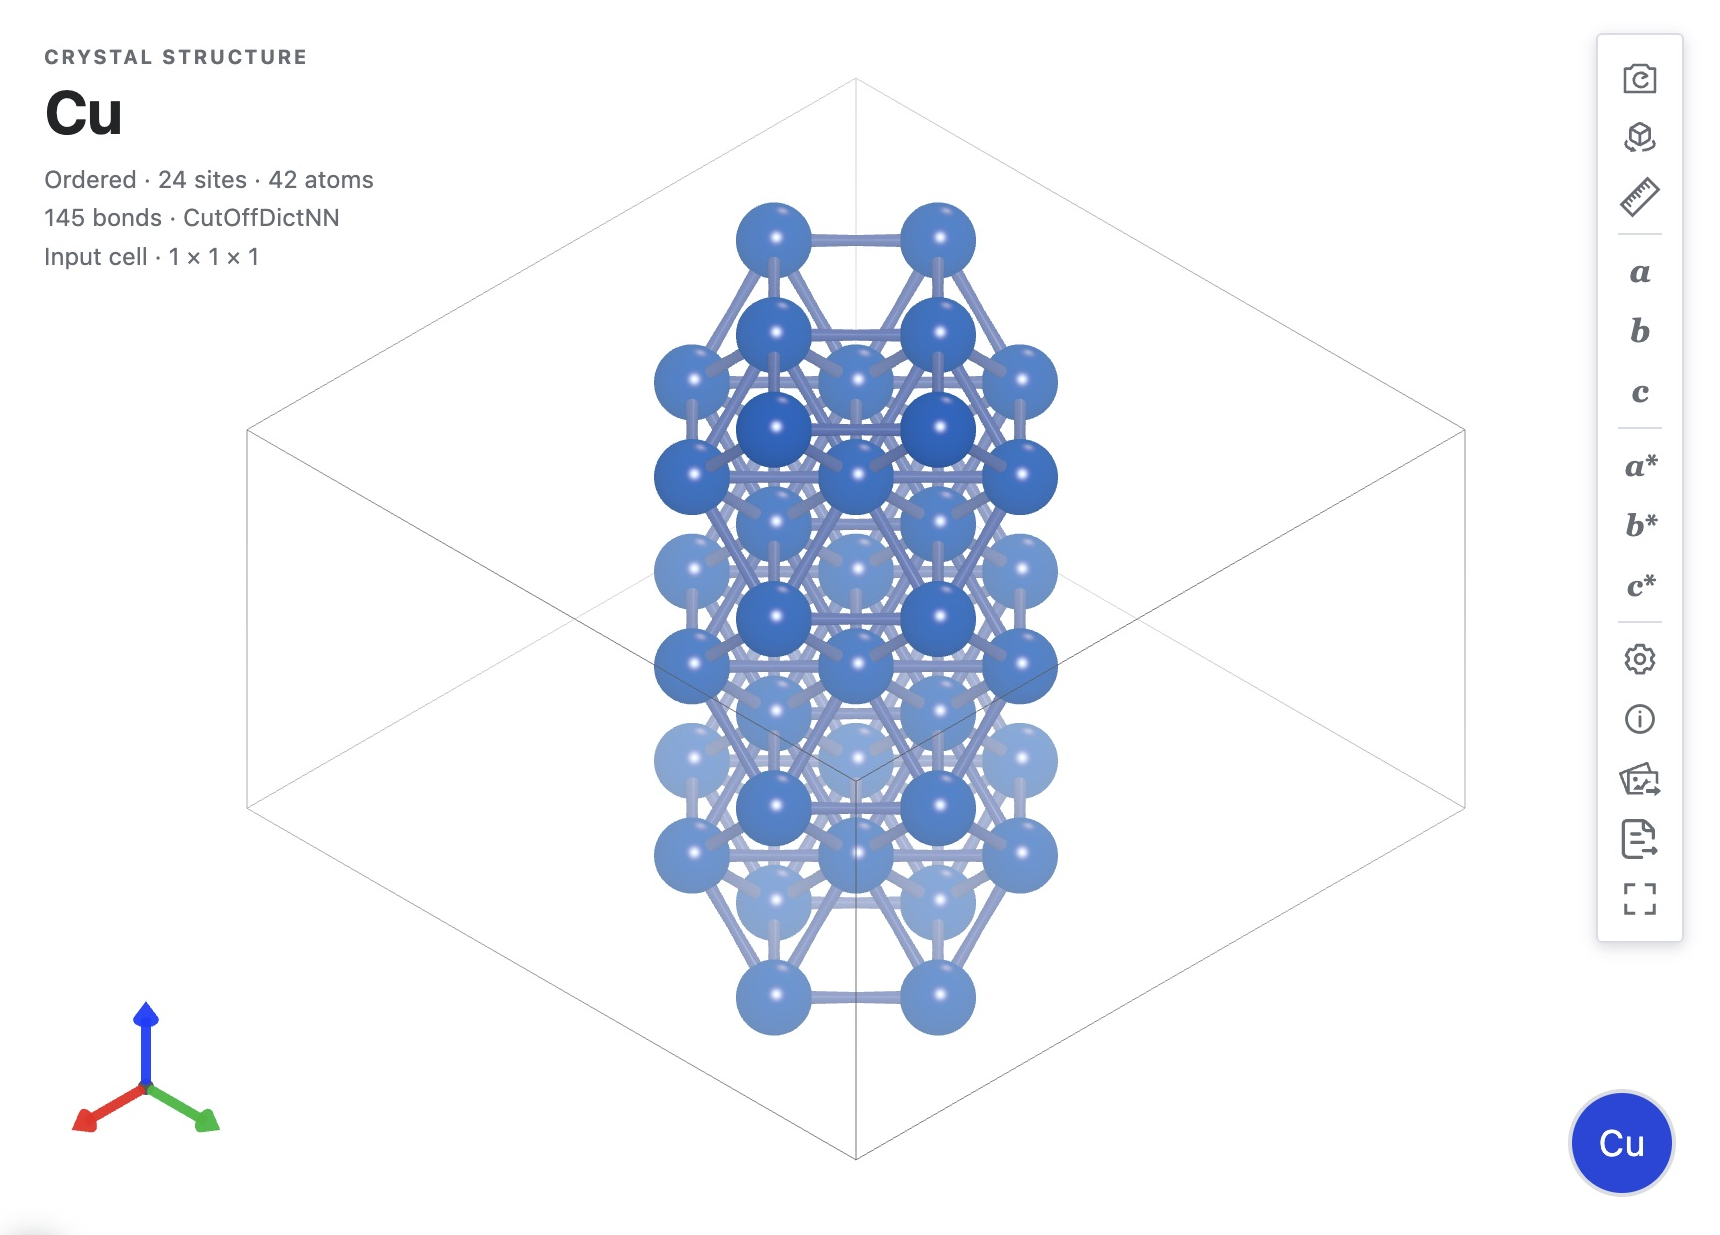
\includegraphics[width=\linewidth]{publication-assets/revision-nanowire-perspective.png}
\caption{隨書24位點銅奈米線的實際顯示。檢視器補出週期邊界原子以展示軸向連線，橫向的空白屬於真空區域。}
\label{fig:nanowire-live}
\end{figure}

\FloatBarrier
\subsection{檢查奈米線的截面與軸向}

開啟隨書\file{Cu-wire-001-r3-l2.json}，即可檢查已經擷取的24位點銅奈米線。它與奈米管都沿$c$方向週期。奈米管由單層捲成空心圓周；銅奈米線保留圓柱範圍內的晶體原子，橫截面內部也有原子。

\begin{steps}
  \item 匯入JSON並開啟三維文件，保持\ui{Input cell}。核對元素為Cu、獨立位點為24。
  \item 單擊檢視工具欄的\ui{c}沿線軸觀察截面。原子排列在離散的晶格位置上，輪廓可以呈階梯狀，不必形成光滑圓邊。
  \item 單擊\ui{a}或\ui{b}看側面，開啟\ui{Unit cell}。用軸向$7.22\,\text{\AA}$與橫向$13.415\,\text{\AA}$的盒長解釋取景：沿軸向是重複週期，橫向大盒用於容納有限截面與真空。
  \item 清除無關選擇，稍微旋轉為同時看見截面和側面的斜檢視。保留晶胞邊框與方位標記，檢查沒有原子被檢視邊緣裁掉。
  \item 按需要將\ui{Repeat cell}的\ui{c}設為2檢視接續，隨後恢復一個週期。儲存專案與結構；匯出圖片時在圖註記錄$[001]$方向、輸入擷取半徑$3\,\text{\AA}$和24個位點。
\end{steps}

輸入半徑決定保留哪些晶格位置，圖中最外原子的跨度則由實際保留的離散位置決定。本例橫向跨度$5.415\,\text{\AA}$小於直徑$6\,\text{\AA}$，與擷取規則一致。後續結構最佳化及電子性質分析可使用相應計算工作流。

\subsection{擷取一個有限銅團簇}
\index{Liangzidian@量子點}

\ui{量子點 / 奈米空洞}的\ui{量子點}模式保留球內原子，建立三個方向均不周期的有限結構。本例用13位點銅團簇觀察有限邊界與週期塊體的區別，儲存後可繼續安排相應的電子結構計算。

\begin{steps}
  \item 重新啟用四位點銅輸入，從\ui{奈米結構}開啟\ui{量子點 / 奈米空洞}。
  \item 處理方式選擇\ui{量子點}，半徑填 $3\,\text{\AA}$，真空層厚度填 $4\,\text{\AA}$，最大原子數設為2000。
  \item 預覽後旋轉觀察，確認沒有一條方向繼續連線成無限原子鏈。檢查共有13個Cu位點。
  \item 應用並命名為\file{Cu-dot-r3}，儲存專案和結構。
\end{steps}

本例的三個胞長均約為 $11.61\,\text{\AA}$，原子在各方向的跨度均為 $3.61\,\text{\AA}$，三向週期標記均為false。最短原子間距約 $2.552655\,\text{\AA}$。按 $2.8\,\text{\AA}$ 的近鄰界限檢查，中心原子有12個近鄰，其餘12個表面原子各有5個近鄰。這一初始團簇從面心立方排列直接裁取，穩定構型需進一步最佳化。

\subsection{在週期銅中挖出球形空洞}
\index{Namikongdong@奈米空洞}

空洞模式保留球外宿主和原週期盒；它與保留球內原子的量子點模式正好相反。先建立足夠大的宿主，可以避免只從很小晶胞中刪去大部分甚至全部原子。

\begin{steps}
  \item 匯入隨書\file{Cu-void-host-2x2x2.json}，或從四位點銅輸入透過\ui{構建超胞}建立 $2\times2\times2$ 宿主。應有32個Cu位點，三個胞長均為 $7.22\,\text{\AA}$。
  \item 啟用這份宿主，開啟\ui{量子點 / 奈米空洞}，處理方式選擇\ui{奈米空洞}，半徑設為 $2.7\,\text{\AA}$。空洞模式不需要為有限團簇增加外部真空。
  \item 預覽並顯示晶胞邊框。空洞中心固定在宿主的分數座標 \((0.5,0.5,0.5)\)，應檢查晶胞中央的原子被移除，而外圍週期宿主仍保留。
  \item 核對本例移除13個原子，剩餘19個Cu位點；晶格仍為 $7.22\,\text{\AA}$ 的立方胞，三個方向繼續週期。
  \item 應用後另存為\file{Cu-void-r2p7}，保留完整32位點宿主，便於以後改變半徑或比較缺陷。
\end{steps}

剩餘原子距空洞中心的最短週期距離為 $3.61\,\text{\AA}$。這個值大於輸入半徑 $2.7\,\text{\AA}$，反映了晶格上可保留的位置是離散的，不表示半徑欄位失效。剩餘宿主的最短原子間距仍約 $2.552655\,\text{\AA}$。儲存時同時記錄“輸入刪除球半徑”和“剩餘最近原子距中心”，會比只給一張透檢視更清楚。

\subsection{檢查週期並儲存配套檔案}

每個例子的原生JSON保留當前晶格、座標、週期標記及相應構建資訊；CIF用於交換晶胞和原子幾何。匯入本組CIF時，三個方向均按週期處理。繼續低維建模並保留本節的週期方向時，應使用JSON。

\begin{table}[htbp]
\centering\small
\caption{隨書奈米結構的位點數與原生週期。}
\begin{tabularx}{\linewidth}{lX}
\toprule
結果 & 實際模型與主要檢查值\\
\midrule
石墨烯奈米帶 & 24C；僅$y$週期；軸向 $8.521690\,\text{\AA}$。\\
$(4,0)$奈米管 & 32C；僅$z$週期；半徑 $1.566085\,\text{\AA}$。\\
銅奈米線 & 24Cu；僅$z$週期；軸向 $7.22\,\text{\AA}$。\\
銅團簇 & 13Cu；三個方向非週期；盒長各 $11.61\,\text{\AA}$。\\
帶空洞的銅 & 19Cu；三個方向週期；32位點宿主中移除13個。\\
\bottomrule
\end{tabularx}
\end{table}

\begin{steps}
  \item 先儲存專案，確認輸入結構和派生結果具有不同名稱。
  \item 如需單獨結構檔案，在檢視器的\ui{Export file}\,$\rightarrow$\,\ui{Structure file}中選JSON，保留模型資訊；幾何交換可另存CIF。這裡不要選擇用於顯示場景的\ui{Scene JSON}。
  \item 重新開啟儲存的結構，檢查位點數、晶胞和週期方向；再檢查邊緣、卷合處或球形裁切邊界的近鄰。
  \item 需要重新生成這組結構時，以\file{-nojvm}啟動MATLAB\regmark{}，配置好工具箱路徑後，從隨書示例目錄執行\file{nano_examples.m}。\file{verify_nano_examples.m}用於檢查已有結構。
\end{steps}

本節提供未鈍化的初始模型，可根據材料與邊界需要繼續鈍化、弛豫和電子結構計算。將模型接入工作流時，儲存構建引數與計算引數，並確認工作流引用所需的結構。
